\documentclass[../main.tex]{subfiles}
\begin{document}

% Allgemeines Kapitel "Sicherheitsuntersuchungen" mit Intro a la:

% Lange Liste an Empfehlungen/best practices für Docker:
%		- einige einfache, die automatisch von Docker erzwungen werden
%		- einige nicht offensichtliche, die manuell aktiviert werden müssen
%		- einige schwierige, die keine Kernel-Unterstützung haben
%	^		\cite[S.10]{presContainerDockerSec}

% Kleinere Angriffsoberfläche für Container durch minimal distros (alpine linux, buildroot, atomic?)
%		- Und durch Tatsache, dass HW-Management komplett auf dem Host gemacht wird, nicht in den Containern
%	^		\cite[S.16]{presContainerDockerSec}

% Immutable Containers mit "docker run --read-only"
%	^		\cite[S.17]{presContainerDockerSec}

% Image Trusting: Imageersteller, Operator der Registry, Transport zwischen Client und Hub
%	^		\cite[S.18]{presContainerDockerSec}

% Security kommt oft mit Usability-Einbußen (was mit Ease of Use eine Stärke von Docker ist)
%	^		\cite[S.26]{presContainerDockerSec}

% Docker Security Zukunft>
%	- noexec, nosuid für immutable containers
%	- bessere GRSEC, PAX, LSM integration
%	- user namespaces
%	- bessere default seccomp profiles
%	^		\cite[S.40]{presContainerDockerSec}

% Zitat vllt mit in eine DockerSecurity Einleitung:
% "A year ago, Docker and security was pretty horrible, six months ago it wasn't so bad, and now it's pretty usable."
% von David Mortman at DEFCON (WELCHES JAHR IST NOCH WICHTIG)
% a la.. "wir untersuchen was er meint, was sich verbessert hat etc."
%	^		\cite[S.41]{presContainerDockerSec}

% Angreifer können ein paar Angriffe ausführen: Privilege escalation und Denial of Service.
%  °	\cite[S.3]{dockerSec1}

\chapter{Sicherheit durch Linux-Funktionen}
\label{secLinux}
	Die Docker-Entwickler haben in den letzten Monaten die Integrations- und Anpassungsmöglichkeiten zusätzlicher Sicherheitsmaßnahmen, v.a. die von Mandatory Access Controls (MACs), stark verbessert, da die Containersicherheit für \emph{Docker} nach eigenen Aussagen höchste Priorität hat \cite{githubDockerRoadmap}\cite{githubDockerChangelog}.

	Auch die Tatsache, dass sich zur Zeit die Konkurrenz \emph{CoreOS} mit der Containerlösung \emph{rkt} als sicherheitsfokusierte Alternative zu Docker auf dem Virtualisierungsmarkt etablieren will \cite{coreosAnnouncementRkt10}, ist Anreiz für \emph{Docker} die Sicherheit ihrer eigenen Entwicklung nicht zu vernachlässigen. Die Veröffentlichung des großen Sicherheitsupdates für Docker mit der Version 1.10 am 4. Februar 2016 geschah wenige Stunden nach der Ankündigung der Version 1.0 von \emph{rkt} seitens \emph{CoreOS} \cite{hnAnnouncementDocker110}\cite{hnAnnouncementRkt10}, was eine starke Konkurrenz zwischen den beiden Anbietern vermuten lässt. % /erkenntlich macht..

	Die allgemeine Vorgehensweise von Docker beruht auf den beiden Prinzipien \emph{Defense In Depth} und \emph{Principle Of Least Privilege}, um einen möglichst sicheren Betrieb von Containern zu ermöglichen.

	\begin{itemize}
			\item \emph{Defense In Depth}: Es werden möglichst viele, unabhängige Sicherheitsschichten kombiniert aktiviert, um die Gesamtsicherheit eines Systems zu erhöhen. Der Funktionsumfang der einzelnen Mechanismen kann sich - wie auch in der vorliegenden Sicherheitsarchitektur von Docker der Fall ist - mit Mechanismen anderer Schichten überschneiden.
			\item \emph{Principle Of Least Privilege}: Die angewandten Sicherheitsmechanismen bewirken, dass die von Docker initiierte Aktionen eingeschränkt werden. Docker ist nur befugt Operationen auszuführen, die dazu dienen, seinen Zweck als Containertechnologie zu erfüllen. Alle anderen Privilegien werden Docker verwehrt.
	\end{itemize}

	% Auf technischer Ebene sind zunächst die grundlegenden Mechanismen zur Isolation und Ressourcenverwaltung zu erwähnen, die das Konzept von Containern ermöglichen. Unter Linux sind das die Techniken Namespaces und Control Groups, von denen Docker, \emph{rkt} und andere Linux-basierten Containertechnologien Gebrauch machen.

	Dieses Kapitel stellt die von dem Betriebssystem Linux und dessen Kernel ermöglichten Sicherheitsmechanismen vor, die Docker im Rahmen dieser beiden Prinzipien unterstützt.

	Dazu zählt die Isolierung kritischer Bereiche, die auf Basis des \texttt{chroot}-Befehls in Form von Namespaces, erfolgt (s. Abschnitt \ref{secIsolierung}). Außerdem werden Control Groups, kurz Cgroups, vorgestellt, die eine Ressourcenverwaltung implementieren (s. Abschnitt \ref{secCgroups}). Während beide Mechanismen eine hohe Sicherheitsrelevanz aufweisen, können sie als featureerweiternde Funktionen eines Hostsystems verstanden werden, deren alleiniges Ziel es ist, die Idee von virtuellen Gastsystemen, den Containern, zu realisieren. %Die in CISSP definierten sicherheitserhöhenden Maßnahmen werden von Namespaces und Control Groups nicht berührt \cite{....}.
	% (TODO): CISSP-Quelle!!

	Anschließend werden Zugriffskontrollen erklärt, die in mehreren Variationen unter Docker existieren (s. Abschnitt \ref{secAccessControls}). Mechanismen dieser Art setzen teilweise Sicherheitsmodelle um, z.B. auf der Basis von sogenannten Capabilities.

	%Auch sind Capability-basierte Sicherheitsfunktionen, wie sie von Linux ermöglicht und in einer Reihe an Werkzeugen Anwendung finden, Gegenstand dieses Kapitels.

	% TODO: Mehr Bezug zur Forschungsfrage schaffen und den Annahmen,Schlussfolgerungen


	Wie in Abschnitt \ref{introVirtContainer} bereits geschildert wurde, wird Docker zur Zeit nur für Linux angeboten. Aus diesem Grund ist eine Untersuchung von Sicherheitsfeatures anderer Betriebssysteme in dieser Arbeit irrelevant.

  % namespaces/etc (was es ist) in Einleitung mit rein? 1.) Erklaeren, 2.) Security/Docker untersuchen dazu im Security Hauptteil
  % 2 Unterkapitel, inhatliche Überschneidung evtl., Grund nennen warum so gegliedert, ...
  % \cite[S.3]{dockerIntroIEEE} --> umgangsprachlich erkleart wie mit namespaces und cgroups gearbeitet wird

	% User namespaces are only one piece of the puzzle. AppArmor/SELinux, Notary, image security, and proper environment/network security all play a part in the overall Docker security picture
	%  ^ 	\cite[S.7]{nsUserContainerCon}

	% Alle vorgestellten Features realisieren Teile des Konzepts "Principle of Least Authority". System ist am sichersten, wenn jedes Subjekt nur minimalen Rechte besitzt, die es benötigt, um Aufgaben auszuführen. Je größer die Menge an eingeräumten Rechten ist, desto größer ist auch das Sicherheitsrisiko eines Missbrauchs \cite[S.722]{tanenbaumOS}.

	\section{Isolierung}
  \label{secIsolierung}
		Die Isolierung für Container wird unter Linux für die meisten kritischen Bereiche eines Systems über Namespaces realisiert.

		Da Anwendungen innerhalb von Container eine komplette Laufzeitumgebung angeboten werden muss, müssen alle relevanten Bereiche des Hostsystems durch Namespaces abgedeckt sein.	Wenn unter Linux z.B. ein neuer Prozess gestartet werden soll, wird dem Kernel über \emph{System Calls} mitgeteilt, hierfür einen neuen Namespace bereitzustellen.

		%Je nach Anforderung gibt es verschiedene Namespaces: PID-, Netzwerk-, Mount-, User- und UTS-Namespace

		%, z.B. ein \emph{network namespace}, der dem neuen Prozess ein Netzwerkinterface zuweist.

		%Um Container als isolierte Arbeitsbereiche auf einem Hostsystem zu erstellen, werden die Namespaces des Kernels verwendet.

		%, sodass neben dem Netzwerk auch z.B. ein beschränkter Zugriff auf den Arbeitsspeicher und die \acrshort{CPU} gewährleistet ist \cite[S.3]{dockerIntroIEEE}.

		Aus technischer Sicht beinhaltet ein Namespace eine Baumstruktur zu betrachtender Ressourcen. Diese Struktur ist in einer Lookup-Tabelle abgebildet, die global verfügbare Ressourcen abstrahiert und innerhalb eines Namespaces bereitstellt. Änderungen globaler Ressourcen sind unsichtbar für Prozesse in einem Namespace, jedoch sichtbar für solche außerhalb. Namespaces sind in der Theorie beliebig verschachtelbar. In der Realität wird diese Eigenschaft durch die Größe der Lookup-Tabelle begrenzt \cite[S.1f.]{IBMcheckpointRestart}\cite{namespaces}.

		Dadurch kann das Konzept von Namespaces als Lösungsansatz betrachtet werden, um das Sicherheitsziel Vertraulichkeit zu erreichen. Sie sind der grundlegende Baustein, um eine Containerisolierung unter Linux zu realisieren. Auch addressieren Namespaces den Punkt (1) aus Abschnitt \ref{questionSolutionTheory}.

		Unter Linux existieren sechs Namespaces, die in die Kategorien IPC, Network, Mount, PID, User und UTS unterteilt sind. Von Docker werden alle verwendet, der User-Namespace jedoch wird erst seit Docker-Version 1.10 unterstützt.

		Es besteht die Möglichkeit, dass bald weitere Namespaces dem bestehenden Set hinzugefügt werden. Zum einen wird derzeit ein eigener Namespace für Control Groups implementiert (siehe Abschnitt \ref{secCgroups}). Zum anderen ist in Diskussion, für die bestehenden Sicherheitsmodule des Kernels (siehe Kapitel \ref{lsm}), diverse Logfunktionen und Geräte unter Linux, eigene Namespaces zur Verfügung zu stellen \cite[S.19]{presContainerSec}.
		% TODO: Mehr Quellen

		% Nach ..(reshetova).. müssen Anforderungen an Prozessisolierung, Dateisystemisolierung, Geräteisolierung, Prozessisolierung und Netzwerklimitierung erfüllt sein.

    % Isolierung erklären, erfüllt X Schutzziele, Bezug auf Forschungsfrage
    % Es gibt 6 Namespaces, die im folgenden *anhand der verschiedenen Betriebssystemkomponenten?) untersucht werden.

		% Unfortunately, the namespace support code is complicated and in the past, various bugs have allowed applications to escape from this namespace isolation and interfere with other containers. The known bugs have been fixed.
		%		^		\cite{ https://coreos.com/blog/container-security-selinux-coreos.html }

		\subsection{Prozessisolierung durch den \acrshort{PID}-Namespace}
		\label{secIsoProcesses}
			% TODO: Offenbar gibts Probleme mit PID=0, da dieser Besonderheiten aufweist (siehe Hackernews Link)

			Jeder Container entspricht auf dem Hostsystem zunächst einem Prozess. Da die Container untereinander isoliert sein sollen, dürfen auch die zugrundeliegenden Containerprozesse nicht miteinander interferieren.

			Docker erreicht diese Isolierung auf Prozessebene durch die Nutzung von PID-Namespaces, in die Container eingebettet werden. Nach diesem hierarchischen Konzept ist es einem Prozess nur möglich, selbsterzeugte Kindprozesse zu beobachten und mit ihnen zu interagieren.

			In \fig \ref{fig:sec_pidNs} ist ein Beispiel von PID-Namespaces gegeben. Ein Prozess besitzt die PID 3698, die außerhalb des rot markierten Namespaces gültig ist. Außerdem besitzt er die PID 1, die innerhalb des Namespaces vergeben wurde. Der Elternprozess mit PID 627 ist in der Lage diesen jederzeit mit dem Befehl \texttt{kill} zu beenden oder allgemein Kindprozesse mit einem Aufruf von \texttt{ps} zu überwachen. Der Prozess mit PID 3698 hingegen befindet sich im roten Namespace und hat keine Kenntnis von der übergeordneten Prozesshierarchie.

			%Elternprozesse, also Prozesse die in der Prozesshierarchie über \emph{8,1} stehen, sind für diesen unsichtbar. Der Elternprozesse haben jedoch die volle Kontrolle über X und können diesen z.B. jederzeit mit dem Befehl \texttt{kill} beenden. Darüber hinaus haben Elternprozesse die Möglichkeit mit z.B. einem Aufruf von \texttt{ps} alle Kindprozesse zu überwachen.

			\vspace{0.5cm}
			\begin{figure}[h]
					\centering
					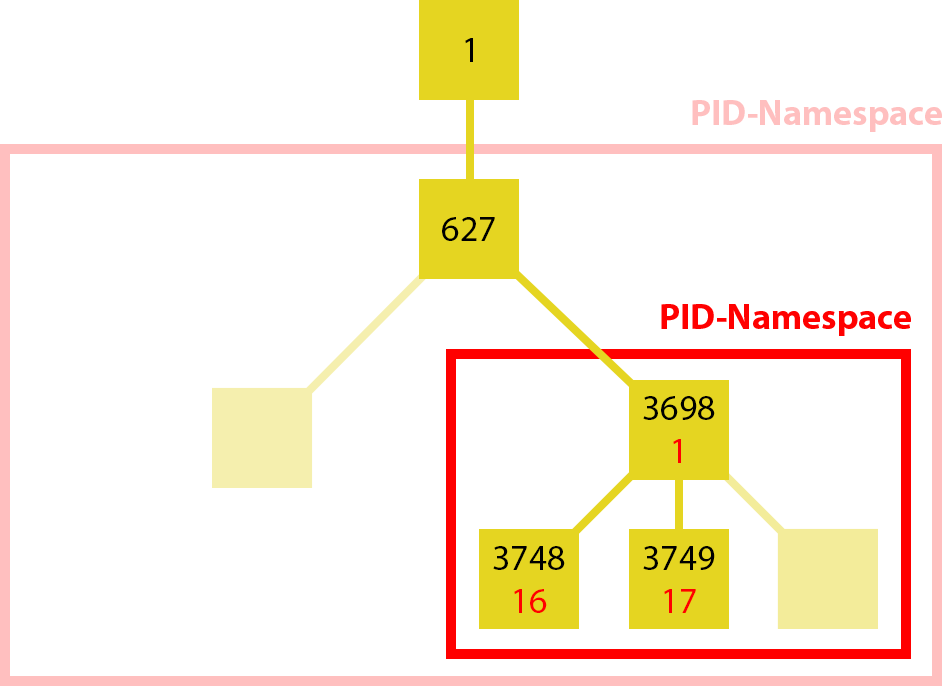
\includegraphics[width=0.9\textwidth]{./images/sec_pidNs.png}
					\caption{Prozesshierarchie unter Verwendung von PID-Namespaces (eigene Abbildung auf Basis von \cite{nsFigures}).}
					\label{fig:sec_pidNs}
			\end{figure}

			Übertragen auf die containerbasierte Virtualisierung bedeutet das, dass das Hostsystem vollen Zugriff auf die laufenden Container hat, Containerprozesse jedoch keine Kenntnis von Prozessen außerhalb des eigenen Namespaces besitzen. Diese Eigenschaft erschwert es Angreifern, ausgehend von \cbroken{}, Schaden anzurichten, da sie keine Informationen über Prozesse außerhalb des eigenen PID-Namespaces erlangen können.

			Ein weiterere nützliche Eigenschaft ist das Setzen der PID auf 1 für einen Prozess, dem ein PID-Namespace zugewiesen wurde. Ein Prozess mit PID 1 ist es möglich, jeder seiner Kindprozesse zu terminieren sobald er selbst beendet wird. Beim Betrieb con Containern kann dieses Feature genutzt werden, um über einen Befehl des Hostsystems einen Container vollständig herunterzufahren.


			%Der initiale Containerprozess kann mit der \texttt{PID=1} gestartet werden, dem es als \emph{init}-ähnlicher Prozess möglich ist, alle Kindprozese zu terminieren sobald er selbst beendet wird. Somit können komplette Container durch einen Hostzugriff auf den Containerprozess mit \texttt{PID=1} umgehend vollständig heruntergefahren werden.

			Wie sich dieses Konzept der Geheimhaltung in der Praxis auf gestartete Docker-Container auswirkt, ist in \fig \ref{fig:sec_pidNsHost} und \fig \ref{fig:sec_pidNsContainer} zu sehen. Zum Vergleich ist die gleiche Situation in obiger \fig \ref{fig:sec_pidNs} dargestellt.

			\begin{figure}[h]
					\centering
					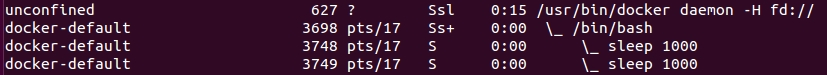
\includegraphics[width=1.0\textwidth]{./images/sec_pidNsHost.jpg}
					\caption{Ausschnitt der Ausgabe des Befehls \texttt{ps -eaxfZ} auf einem Docker-Hostsystem (eigene Abbildung).}
					\label{fig:sec_pidNsHost}
			\end{figure}
			% TODO: lstlisting hieraus machen bzw. Screenshot mit "BlackOnWhite"-Colorsetting des Terminals machen (gilt fuer alle Terminal Screenshots!)

			\begin{figure}[h]
					\centering
					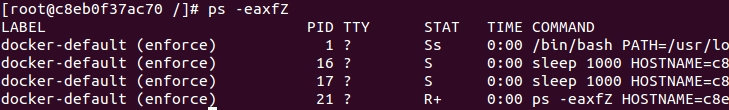
\includegraphics[width=1.0\textwidth]{./images/sec_pidNsContainer.jpg}
					\caption{Ausgabe des Befehls \texttt{ps -eaxfZ} in einem Docker-Container (eigene Abbildung).}
					\label{fig:sec_pidNsContainer}
			\end{figure}

			\fig \ref{fig:sec_pidNsHost} zeigt einen Auschnitt der Ausgabe des Befehls \texttt{ps -eaxfZ} auf dem Hostsystem. Er enthält die laufenden Docker-Prozesse des Daemons mit PID 627 (Zeile 1) sowie die eines Containers, in dem eine Shell gestartet wurde (Zeile 2). Innerhalb der Shell wurde der Befehl \texttt{sleep 1000} zweifach ausgeführt, was die Erstellung zweier neuer Prozesse zur Folge hat (Zeile 3 und 4). Wie zu erkennen ist, sind die einzelnen Containerprozesse aus Sicht des Hostsystems identifizierbar.

			% TODO: lstlisting hieraus machen bzw. Screenshot mit "BlackOnWhite"-Colorsetting des Terminals machen (gilt fuer alle Terminal Screenshots!)

			\fig \ref{fig:sec_pidNsContainer} zeigt die vollständige Ausgabe des gleichen Befehls innerhalb eines Containers. Prozesse außerhalb des Containers sind nicht sichtbar. Außerdem weisen die Containerprozesse im Vergleich zu \fig \ref{fig:sec_pidNsHost} nun eine andere PID auf. Da die Shell der initiale Containerprozess ist, erhält sie die PID 1.

			% PID namespaces sind hierarchisch http://lwn.net/Articles/259217/

			% Einzelnen Containerlösungen unterscheiden sich nur geringfügig. Alle nutyen namespace, cgroups, chroot.
			% Unterschiede im Contaier lifecycle jedoch (docker sehr gut aufgestellt --> teil von dockers erfolg beruht darauf)
			%	^		\cite[S.4]{virtVSContainer}

    \subsection{Dateisystemisolierung durch den Mount-Namespace}
			Auch das Dateisystem des Hostsystems \(h\) muss vor unrechtmäßigen Zugriffen aus einem Container \cbroken{} geschützt werden.

			Allgemein ist ein Dateisystem, wie eine Prozessstruktur in Abschnitt \ref{secIsoProcesses}, hierarchisch aufgebaut. Erstgenanntes kann mithilfe des Mount-Namespace unterteilt werden, sodass unter Docker jeder Container eine andere Sicht auf die Verzeichnisstruktur des Hostsystems hat. Nur ein bestimmtes Unterverzeichnis ist für einen Container sichtbar, wenn er dieses als Mountpoint einbindet.

			Das virtuelle \texttt{/proc}-Verzeichnis des Hostsystems bleibt von Mount-Namespaces unberührt, da es essentielle Informationen für jeden Prozess enthält \cite{creatingContainers}\cite{secPart1}. Außerdem erfordern Anwendungen, die innerhalb von Containern laufen, Zugriff auf besagtes Verzeichnis. Als Konsequenz erben Container diese notwendigen Verzeichnisse direkt von ihrem Host.

			Es enthält aber auch Details des Kernels und anderer Prozesse \cite{proc}. Diese müssen wegen der Existenz von \cbroken{} vor Lese- und Schreibzugriffen geschützt werden. Linux erlaubt es, Verzeichnisse derart freizugeben, dass Prozesse nur lesend mit ihnen in Verbindung treten können. Docker unterstützt das standardmäßige Einbinden ohne Schreibrechte \cite[S.4f.]{dockerSecIntro}.


			%Einige Verzeichnisse des Hostsystems werden nicht in den Mount-Namespace einbezogen. Sie werden für den Betrieb von Docker-Containern nicht benötigt und enthalten teilweise kritische Informationen,

			%Dazu gehören die Verzeichnisse:

			%\begin{itemize}
				%\item \texttt{/sys}:
				%\item \texttt{/proc/sys}:
				%\item \texttt{/proc/sysrq - trigger}:
				%\item \texttt{/proc/irq}:
				%\item \texttt{/proc/bus}:
			%\end{itemize}
			% TODO: Quelle

			% Docker dämmt dieses Risiko ein, indem es nur einen reinen Lesezugriff ohne Schreibrechte auf diese Verzeichnisse erlaubt \cite[S.4]{dockerSecIntro}.

			Einem Containern ist es nicht erlaubt, Verzeichnisse des Hostsystems erneut einzubinden. Dieses Verbot wird technisch über die Verweigerung der Capability \texttt{CAP\_SYS\_ADMIN} (s. Abschnitt \ref{capabilities}) erreicht. Ist ein Container im Besitz dieses Rechts, kann dieser Verzeichnisse, deren Zugriff ihm ursprünglich nur lesend gestattet wurde, neu einbinden. Im Rahmen des neuen Mountvorgangs, kann der Container über die Zugriffsart auf einzubindenen Verzeichnisse frei verfügen und ist nicht allein auf das Leserecht beschränkt.


			%, um unrechtmäßige Schreibrechte auszuschließen. Dieses Verbot wird durch die Verweigerung der Capability \texttt{CAP\_SYS\_ADMIN} für Container erreicht.
			% TODO: Einbinden: Dateisysteme werden gemountet unter der Angabe der Berechtigung, also ob read oder write. EIn remount ist daher gefährlich.

			Mit dem Konzept von Mount-Namespaces interferieren Daten von Containern nicht. Jede oberste, beschreibbare Schicht eines Containers wird in einem speziell dem Container zugewiesenen Verzeichnis gespeichert. Unter der Annahme, dass es sich bei Mount-Namespaces um ein sicheres Verfahren handelt, kann ein \cbroken{} nicht in Verzeichnisse anderer Container aus \(C\) schreiben.

			% TODO: LSMs tragen hierzu auch bei! erwaehnen
			% .... nahhh.. besser in LSM-Kapitel erwaehnen, dass LSMs Namespaces verstaerken und weiter absichern


			%Durch die in \ref{dockerContainer} beschriebene, eigene Schicht von Containern
			%Durch das von Docker genutzte, bereits in Kapitel \ref{dockerImages} beschriebene \emph{\acrshort{COW}}-basierte Dateisystem, ist es jedem Container möglich, Änderungen in seinem durch den \emph{mount namespace} zugewiesenen Verzeichnis zu speichern. Containerdaten interferieren dadurch nicht und sind containerübergreifend nicht sichtbar, auch beim Betrieb von Containern, die auf einem gleichen Basisimage beruhen \cite[S.4]{dockerSecIntro}.

			% Filesystem Isolation kann mit user namespaces verstaekrt werden, indem user und groups IDs auf wenige rpriveliigierte host uids und group ids gemappt werden. Zusammen mit dem mount namespace und einer pivot_root umgebung kann das den schutz fuer filesystembasierte Attacken erhoehen
			%		^ 	\cite[S.11]{dockerSec2}


    \subsection{\acrshort{IPC}-Isolierung durch den \acrshort{IPC}-Namespace}
			Ergänzend zu den PID-Namespaces, die die Sichtbarkeit sowie Kontrolle über Prozesse in der Prozesshierarchie einschränken, kann auch die Kommunikation zwischen Prozessen, die \gls{InterProcessCommunication}, limitiert werden. Für diesen Zweck erlaubt Linux die Erstellung von IPC-Namespaces.

			% TODO: Quelle



			Docker gewährleistet dies durch die standardmäßige Zuweisung eines IPC-Namespaces pro Container, in dem ein Prozesse nur mit anderen Prozessen in Kontakt treten kann, wenn sich diese im gleichen IPC-Namespace befinden. Eine versehentliche oder beabsichtige Interferenz zwischen Containern oder zwischen Containern und Docker-unabhängigen Prozessen des Hostsystems wird damit ausgeschlossen.

			%Fast alles bisher:
			%\cite[S.4]{dockerSec1}

			% Problem mit TIPC Extension, wo ipc namespace umgangen werden kann
			%		^ 	\cite[S.18]{dockerSec2}

    \subsection{Netzwerkisolierung durch den Network-Namespace}
			Um einen sicheren Betrieb von Docker zu gewährleisten, müssen Container so konfiguriert sein, dass sie weder den Netzwerkverkehr des Hostsystems noch den anderer Container abhören oder manipulieren können.

			Dazu stellt Docker jedem Container einen eigenen unabhängigen Netzwerkstack zur Verfügung, der durch Network-Namespaces realisiert wird. Jeder Namespace hat seine eigene private \acrshort{IP}-Adresse, IP-Routingtabelle, Loopback-Interface und Netzwerkgeräte \cite[S.2f.]{virtVSContainer}. Eine Kommunikation zu anderen Containern auf dem gleichen oder entfernten Hosts geschieht nur über dafür vorgesehene Schnittstellen.

			Um die oben genannten Netzwerkressourcen anzubieten, wird jedem Network-Namespace ein eigenes \texttt{/proc/net}-Verzeichnis zugewiesen, das netzwerkspezifische Informationen enthält \cite{proc}. Die Nutzung von Befehlen wie \texttt{netstat} und \texttt{ifconfig} wird damit aus einem Network-Namespace heraus auch ermöglicht \cite[S.7]{IBMcheckpointRestart}.

			Standardmäßig wird von Containern eine \emph{Virtual Ethernet Bridge} mit dem Namen docker0 genutzt, um mit dem Hostsystem und anderen Containern zu kommunizieren. Neu gestartete Container werden dieser Bridge hinzugefügt, indem deren Netzwerkinterface \emph{eth0} mit der Bridge verbunden wird. Aus Sicht des Hostsystems ist das Interface \emph{eth0} ein virtuelles \emph{veth}-Interface. Angepasste Netzwerktreiber können für Bridges und sogenannte Overlaynetzwerke, die eine Kommunikation zwischen mehreren Docker-Systemen ermöglichen, erstellt und genutzt werden \cite[S.3]{virtVSContainer}\cite{dockerNetworking}. Aus Gründen der Netzwerksicherheit macht es Sinn eigene Treiber zu verwenden, da die standardmäßige Bridge ohne Filter operiert. Filter können z.B. mit dem Programm \emph{ebtables} erstellt werden.
			% Erklärungen von John:
			% MAC-Flooding: ARP-Tabelle des Opfers wird überfüllt mit falschen Informationen. Angreifer sendet dazu falsche, unterschiedliche ARP-Daten an Opfer, die letzteres in eigenen ARP-TAbelle aufnimmt. Andere Netzteilnehmer (legitime) erreichen das Opfer nicht mehr, da dessen ARP-Tabelle voll ist. Es gibt Angreifer-Tools, die ARP-Pakete vor dem Senden beliebig aendern können (IP und MAC), sodass unique ARP-Eintrag im Zielrechner dazukommt
			% 		--> Verfügbarkeit, DoS
			% ARP-Spoofing: ARP-Tabelle wird gezielt manipuliert, also einzelne Einträge. Z.B. sendet Angreifer Gratitiuous ARP raus, um bekanntzugeben, dass Gateway mit IP X jetzt unter neuer MAC zu erreichen ist, also seiner eigenen z.B. Wenn richtig gemacht, kann dann Angreifer kompletten Traffic der Zielrechner als MITM mitlesen.
			%			--> Wenn nicht weiergeleitet: Verfügbakrit/DoS. Wenn weitergeleitet: Vertraulichkeit, Integrität


			%Die Bridge leitet ohne Filter alle eingehenden Pakete weiter, welchen Umstand dieses Verbindungsdesign anfällig gegenüber \acrshort{ARP}-Spoofing und \acrshort{MAC-NET}-Flooding macht. Diesem Nachteil kann Abhilfe geschafft werden, indem manuelle Filtermethoden mittels beispielsweise \emph{ebtables} in die Bridge integriert werden, oder ein anderes Verbindungsdesign auf basis virtueller Netzwerke gewählt wird.
			% todo: Im Glossar die beiden Angriffe erklären?
			% todo: ebtables besser erklaeren falls noch relevant http://ebtables.netfilter.org/

			% TODO: Bild zu Bridge-Layout (z.B. in dockerSec1, s.5, oben)

			% TODO: Integrieren: https://docs.docker.com/engine/userguide/networking/

			%Fast alles bisher:
			%\cite[S.4]{dockerSec1}

			% network namespace:
	    % Standardmäßig werden für Container keine Ports geöffnet. Manche Applikationen machen jedoch nur Sinn, wenn sie Ports nutzen können, daher können diese manuell in dem Dockerfile (INTERNE REFERENZ) freigegeben werden.
	    % Container werden virtuelle Netzwerkinterfaces zur Verfügung gestellt. Dadurch können z.B. mehrere Container betrieben werden, die Webserver beinhalten, die alle auf Port 80 eingestellt sind. Außerhalb der Container können diese Containerports mithilfe von NAT (sicher NAT?) auf unterschiedliche Ports des Hosts abgebildet werden.
	    %  ^ \cite[S.3]{dockerIntroIEEE}

    \subsection{Userisolierung durch den User-Namespace}
			Bislang werden Container unter Docker und anderen Containerlösungen mit Rootrechten gestartet. Falls es einem Angreifer in diesem Szenario gelingt, aus der Isolierung von \cbroken{} auszubrechen, ist er automatisch Root-User auf dem Host, was ein hohes Sicherheitsrisiko birgt. Durch die potentielle Gefahr dieser Vorgehensweise, ist die Einführung von User-Namespaces mit Docker-Version 1.10 ein Meilenstein für die Sicherheit von Docker.
			% Quelle hinzufuegen .. blog artiekl etc.
			% schlechte Quelle...: http://rhelblog.redhat.com/2015/07/07/whats-next-for-containers-user-namespaces/
			% Root-Rechte wurden bisher mit capabilities eingeschränkt.

			Dieser Namespace führt einen Mechanismus ein, unter dem Rootrechte in Containern nicht Rootrechten auf dem Hostsystem entsprechen. Ein Root-User innerhalb eines Containers wird auf dem Hostsystem auf einem Nicht-Root-User abgebildet.

			Linux verwendet User-IDs (UIDs) und Group-IDs (GIDs), um Verzeichnisse und Dateien eines Dateisystems sowie Prozesse mit Eignerinformationen zu versehen. User-Namespaces erlauben unterschiedliche UIDs bzw. GIDs innerhalb und außerhalb des Namespaces. Im Kontext des Hostsystems kann dadurch ein unpriveligierter User ohne Rootrechte existieren, während der gleiche User innerhalb von Containern mithilfe von User-Namespaces priveligiert ist \cite{nsUser}.

			%In der Praxis lassen sich mit diesem Konzept jeweils Root-User mit UID 0 in Container X und Y auf nicht-priviligierte User, z.B. mit \texttt{uid=1000} und \texttt{uid=2000} des Hosts, abbilden.
			% TODO: Grafik zur Unterstuetzung waere gut hier...

			Eine Unterstützung von User-Namespaces war seit Docker-Version 1.6 vorgesehen \cite{githubUserNamespaceProposal}. Durch einen Bug der Programmiersprache \emph{Golang} und Integrationschwierigkeiten in die bestehende Docker-Codebasis, kam es jdoch zu Verzögerungen \cite{nsUserGolangBug}\cite{githubUserNamespaceConflict}\cite{githubUserNamespaceIntegration}. Beide Probleme sind jedoch mittlerweise behoben, wie die erfolgreiche Integration von User-Namespaces in aktuelle Releases von Docker bestätigt \cite{githubUserNamespaceIntegration}. In der aktuell neusten Docker-Version 1.10 werden besagte Namespaces nicht automatisch verwendet. Sie müssen manuell, wie z.B. in \cite{nsUserEnable} erklärt, aktiviert werden \cite{githubDockerChangelog}. Eine standardmäßige Verwendung des Namespace ist in Zukunft zu erwarten.

			% Mehr (Bessere) Gruende: http://events.linuxfoundation.org/sites/events/files/slides/User%20Namespaces%20-%20ContainerCon%202015%20-%2016-9-final_0.pdf
			% S.13ff.

			% A single-threaded process can join another user namespace with setns(2) if it has the CAP_SYS_ADMIN in that namespace; upon doing so, it gains a full set of capabilities in that namespace.
			%		^ 	\cite{nsUser}

      % \texttt{user namespaces} ist Future implementation, da neues Kernelfeature. Trotzdem Konzept erklären und wie Docker-Security davon profitiert.

			% User namespace is the only namespace which can be created without CAP_SYS_ADMIN capability
			% aus: http://www.haifux.org/lectures/299/netLec7.pdf .... Seite 61

			Auch für Cloudanbieter sind User-Namespaces von Vorteil: Mit einer Auflösung der Container auf Userebene ist es möglich die Nutzung von Diensten auf Userbasis einzugrenzen und abzurechnen \cite[S.3]{nsUserContainerCon}.

		\subsection{\acrshort{UTS}-Isolierung durch den \texttt{\acrshort{UTS}-namespace}}
			Mit einem \emph{\acrshort{UTS}-namespace} ist es möglich, jedem Container einen eigenen Hostnamen zuzuweisen. Der Container kann diesen Namen abfragen und ändern \cite[S.3]{virtVSContainer}. Dieser Namespace trägt damit nicht zur Containersicherheit bei und ist daher nur aus Gründen der Vollständigkeit an dieser Stelle erwähnt.

		\subsection{Geräteisolierung}
			% Es gibt keinen richtigen Namespace dafuer, da linux device driver (die physischen devices kontrollieren), nicht namespace aware sind und damit nicht sicher in containern verwendet werden koennen
			% Nur die Cells-Implementierung baut einen 'device namespace'
			% Sonst nur ueber capabilities einschraenkbar (gennant im text: CAP_SYS_MKNOD)
			%		^ 	\cite[S.12]{dockerSec2}

			In Unix-basierenden Betriebssystemen wie Linux erfolgt der Zugriff auf Hardware über sogenannte Device Nodes (Geräte), die im Dateisystem von speziellen Dateien repräsentiert sind.
			% TODO: Device Nodes ins Glossar aufnehmen. Dort dann sagen, dass es speyielle Files sind etc.

			Ein paar wichtige Geräte und deren Zuständigkeiten sind im Folgenden aufgeführt. Das Netzwerkinterface ist auch ein Gerät, welches bereits mit dem Network-Namespace isolierbar ist \cite{deviceNs}.

			\begin{itemize}
				\item \texttt{/dev/mem}: Arbeitsspeicher
				\item \texttt{/dev/sd*}: Dateien für den Zugriff auf Speichermedien
				\item \texttt{/dev/tty}: Terminal
			\end{itemize}

			Wie zu sehen ist, handelt sich dabei um kritische Systemkomponenten, über die Container unter keinen Umständen verfügen dürfen. Deswegen ist es notwendig den Zugriff auf Geräte stark einzuschränken, um den Host vor Missbrauch zu schützen.
			% (TODO): Starke Abhängigkeit zu cgroups (guten Übergang machen bzw. Abgrenzung)

			Aktuell existiert im Linux-Kernel kein eigener Namespace für Geräte. Die Implementierung von Device-Namespaces erfolgte bereits von \emph{Cellrox}-Mitarbeitern im Jahr 2013 \cite{deviceNsCerrox}. Eine Integration in den Linux-Kernel fand jedoch bislang nicht statt.

			Docker löst dieses Problem, indem es standardmäßig den Zugriff auf Geräte von unpriveligierten Containern untersagt. Über die Befehlssyntax \texttt{docker run --device=DEVICE} können auch unpriveligierten Containern Geräte manuell zur Verwendung freigegeben werden. Priveligierte Container können beliebig auf Geräte zugreifen \cite{dockerRun}.



			% Standardmaessig haben Container keinen zugriff auf Devices. Kann aber explizit bei container launch anders festgelegt werden \cite[S.4]{dockerSecIntro}

			% Problem mit PseudoRandomNumberGenerator in /dev/random und /dev/urandom, da das blocking devices sind
			%		^ 	\cite[S.18]{dockerSec2}

			% Problem mit HotPlug Support unter Linux
			%		^ 	\cite[S.19]{dockerSec2}

	\section{Ressourcenverwaltung durch Control Groups}
  \label{secCgroups}
		\acrshort{DoS}-Angriffe beabsichtigen das Sicherheitsziel der Verfügbarkeit zu verletzen und gehören in \gls{MultiTenantService}-Systemen zu einem verbreiteten Angriffsmuster \cite[S.5]{dockerSec1}. Um die Verfügbarkeit von Containern sicherzustellen, bietet der Linux-Kernel sogenannte Control Groups (\acrshort{cgroups}) an.

		Alle gängigen Linux-basierten Containerlösungen, darunter auch Docker, nutzen aktuell Control Groups, um Ressourcen für Container zu verwalten \cite[S.16]{dockerSec2}. Der Einsatz von Cgroups unter Docker umfasst - wie im Quellcode von \emph{runC} zu sehen ist - die Kontrolle über \acrshort{CPU}, Arbeitsspeicher, Geräte, Netzwerkinterfaces und \acrshort{I/O}-Operationen auf Speichermedien wie \acrshort{HDD}, \acrshort{SSD} und \acrshort{USB}-Speicher \cite{cgroupsRedhat}\cite{githubRunCCgroups}. Die Verwaltung von Letzteren wurden mit dem neusten Docker-Release, Version 1.10, erweitert \cite{docker110}.

		% \emph{control groups}, oder auch verkürzt \emph{cgroups} genannt, ist hierbei das Schlüsselfeature des Linuxkernels, um dieser Art von Angriff entgegenzuwirken. Sie stellen sicher, dass jeder Container nur begrenzt Hostressourcen beansprucht. Mit Docker lassen sich Limits und Bedingungen individuell pro Container anpassen, z.B. an einen bestimmten Container gerichtetes Arbeitsspeicherlimit in Bytes, das ihm maximal im Betrieb zur Verfügung steht \cite[S.4]{dockerSecIntro}.
		% --> Quelle aus docker docs findbar?

		Über die Kommandozeile lässt sich der \texttt{run}-Befehl, der ausgeführt wird, um einen Container zu starten, mit Angaben zur Ressourcennutzung parametrisieren. Z.B. bewirkt die Hintereinanderausführung folgender Befehle, dass dem zuletzt gestarteten Container doppelt so viel CPU-Leistung zur Verfügung gestellt wird, wie dem ersten Container \cite{dockerRun}.

		\begin{lstlisting}
			user@machine:$ docker run IMAGE --cpu-shares=50
			user@machine:$ docker run IMAGE --cpu-shares=100
		\end{lstlisting}

		Neben dem Ressourcenmanagement bieten Control Groups auch Nutzungsstatistiken an. Diese sind unter Docker mit dem Befehl \texttt{docker stats CONTAINER [CONTAINER]} für ein oder mehrere Container abrufbar \cite{dockerMetrics}.

		Control Groups sind historisch aus dem Konzept von sogenannten Ressource Limits, auch Rlimits genannt, gewachsen. Mit Ressource Limits werden \gls{weicheHarteLimits} definiert, die jedem Prozess zugewiesen werden. Der Betrieb von Containern verlangt jedoch eine Ressourcenverteilung auf Containerbasis. Wie in Abschnitt \ref{secIsoProcesses} gezeigt wurde, entspricht ein Container einem Set an Prozessen.
		% TODO: rlimits abgleichen mit \cite[fundamentalkapitel]{linuxInterface}

		%Dieses minimale Konzept auf Prozessebene ist für den Betrieb moderner Container jedoch unzureichend, da u.a. keine Beschränkungen auf Containerebene, also für Prozessgruppen, vorgenommen werden können. % z.B. keine Aktionen festgelegt werden können, die ausgeführt werden, wenn ein solches Limit erreicht ist. Außerdem können die \acrshort{CPU} und der Speicher nur begrenzt von \emph{\acrlong{rlimits}} kontrolliert werden.

		Viele Containertechnologien erweiterten deswegen Resource Limits mit eigenen Features. Z.B. fügten die Entwickler von \emph{FreeBSD} für den Betrieb von \emph{Jails} sogenannte \emph{Hierarchical Resource Limits} hinzu \cite{freeBsdRCTL}. \emph{Solaris} bietet die Nutzung von \emph{Resource Pools} an, die eine Partitionierung von Ressourcen implementieren \cite{cgroupsUniHierarchyDoc}. Auch \emph{OpenVZ} und \emph{Linux-VServer} erweitern die Ressource Limits, sodass weiche und harte Limits pro Container definiert werden können \cite[S.15f.]{dockerSec2}.

		Die Nachteile von Ressource Limits wurden mit der Implementierung von Control Groups für den Linux-Kernel behoben. Mit diesem relativ neuen Mechanismus werden Prozesse in hierarchischen Gruppen angeordnet, die individuell verwaltet werden und deren Attribute vererbt werden können. Neben vielseitiger und feingranularer Funktionen zum Management von z.B. CPU- und Speicherressourcen, können unter Control Groups komplexe Verfahren implementiert werden, die zur Korrektur von limitüberschreitender Prozesse dienen \cite{cgroupsRedhat}. Die Implementierung von Control Groups wurde ab 2012 weiter verbessert, sodass eine Update unter dem Namen \emph{Unified Control Group Hierarchy} im Jahr 2014 in den Linux-Kernel integriert wurde \cite{cgroupsFixing}\cite{cgroupsUniHierarchy}. Von Docker wird dieses Update noch nicht verwendet \cite{githubCgroupsUniHierNotSupported}. In zukünftige Kernelversionen soll ein neuer Control Groups-Namespace implementiert werden, der auf der \emph{Unified Hierarchy} basiert \cite{cgroupNs}.

		Wichtig zu erwähnen ist, dass die Implementierung von Control Groups, verglichen mit der von Ressource Limits, angeblich nicht vollständig ist. Das Feature, Dateisysteme als Ressourcen mit Control Groups zu steuern, fehlt nach Aussagen von Reshetova et al. \cite[S.19]{dockerSec2}. Auch im aktuellen Quellcode von \emph{runC} ist eine Schnittstelle zum Dateisystem als \glqq{}nicht unterstützt\grqq{} gekennzeichnet und wird demzufolge auch nicht von Docker genutzt \cite{githubRunCCgroups}. Diskussionen im \emph{GitHub}-Repository von Docker verweisen in Bezug zu diesem Feature auf Abhängigkeiten zur Art des Dateisystems. Offenbar lassen sich Kontingente für die Nutzung von Dateisystemen nur mit \emph{Device Mapper} und \emph{Brtfs} softwaretechnisch lösen. \emph{AuFS} ermöglicht dieses Feature hingegen nur indirekt über die Zuweisung von Festplattenpartitionen fester Größe. Diese Gegebenheit lässt vermuten, dass eine universelle Lösung aktuell an der Breite unterstützter Dateisysteme scheitert \cite{githubDockerIssueFsQuota}. Die neusten Entwicklungen sehen jedoch eine Implementierung von Kontingenten vor \cite{githubDockerPullBrtfs}.

		Es ist zu erwarten, dass die fehlenden Funktionen von Control Groups sowie die ausstehende Unterstützung der \emph{Unified Hierarchy} zukünftig im Rahmen der Integration des Control Groups-Namespace stattfindet.
		%Eine weitere einheitliche Verwaltung von Ressourcen auf der Basis von Control Groups ist vorgesehen \cite[S.16+19]{dockerSec2}.

		Für Docker-Version 1.11 wurde außerdem die Unterstützung von \acrshort{PID}-Control Groups angekündigt. Sie sollen ergänzen zu den bereits unterstützten Ressourcentypen die Anzahl der erlaubten Prozesse innerhalb eines Containers regulieren \cite{githubCgroupPID}\cite{docker110Security}. Dieses Update verhindert das Angriffsmuster sogenannter \glspl{ForkBomb}.
		% TODO: Abgleichen mit ... Local DoS: Fork-bomb (siehe \cite[S.793]{linuxInterface})

		% TODO: Evtl. stress test aus
		% https://goldmann.pl/blog/2014/09/11/resource-management-in-docker/
		% nachmachen. Da sieht man wie CPU geteilt wird.

		% Was nur rlimits, aber nicht cgroups koennen: filesystem und number of threads verwalten.
		% --> Hängt das zusammen mit "cgroups nocht nicht vollständig implementiert" ?
		%		^		\cite[S.15]{dockerSec2}
		% Mit einer Kombination von \texttt{\acrshort{cgroups}} und \texttt{\acrshort{rlimits}} können Ressourcen der CPU, dem Arbeitsspeicher und dem Dateisystem sowie Festplatten-\acrshort{I/O} effektiv begrenzt werden
		% in dem satz disk IO ins glossar machen? anstelle von festplattenzugriffs

		% (TODO): Quota support im dateisystem noch nicht moeglich https://github.com/docker/docker/issues/3804

    % Sicherheitsziel: Availability, Bezug auf Forschungsfrage

		% "Device Whitelist Controller" feature von cgroups limitiert Set an Devices, die Docker-Container nutzen dürfen.
		%  ^ \cite[S.4, rechts oben]{dockerSec1}

		% cgroups sind noch nicht vollstaendig implementiert (noch nicht alles features von vorgaenger rlimits in cgroups uebernommen)
		%		^ 	\cite[S.19]{dockerSec2}

		% 2. 'docker update' command, although I would have preferred 'docker limit'.
		% 	Ability to change container limits at runtime:
		%		- CPUQuota - CpusetCpus - CpusetMems - Memory - MemorySwap - MemoryReservation - KernelMemory
		%		With this feature in place, there is no reason to run containers without limits, at least memory limits.
		%		^		\cite{https://news.ycombinator.com/item?id=11037543} und release notes von docker v.1.10 ... angeblich ein 'docker update', mit dem memshare,cpushares,etc. zur laufzeit von containern angepasst werden koennen.

		% Neu geplant in V.1.11: PID cgroups http://blog.docker.com/2016/02/docker-engine-1-10-security/
		% neu mit Version 1.11: PID cgroups
		% https://blog.docker.com/2016/02/docker-online-meetup-33-security/	..... mit github issue link
		% verhindert fork bombs

  \section{Einschränkung von Zugriffsrechten}
		\label{secAccessControls}

		Auf Basis der in \ref{questionEffects} erarbeiteten Annahme, dass Angreifer ausgehend von \cbroken{} Angriffe gegen die Sicherheitziele von \(h\) und \(C\) ausüben kann, müssen weitere Sicherheitsmechanismen verwendet werden, um letztere zu schützen. Diese zusätzlichen Mechanismen realisieren Zugriffskontrollen, die auch dann die Sicherheit von \(h\) und \(C\) wahren, wenn es einem Angreifer möglich ist, seine Privilegien in \cbroken{} unrechtmäßig auszudehnen.

		Die in diesem Kapitel vorgestellten Maßnahmen zur Zugriffskontrolle addressieren Punkt (2) des Lösungsansatzes aus Abschnitt \ref{questionSolutionTheory}.

		Zunächst werden zwei grundsätzliche Sicherheitsrisiken von Betriebssystemen, insbesondere Linux, vorgestellt, die in diesem Kapitel mit geeigneten Lösungsansätzen addressiert werden.

		\begin{itemize}
			\item	Wie die regelmäßige Entdeckung neuer Schwachstellen zeigt, sind Programmierfehler in Anwendungen und im Kernel nicht auszuschließen. Eine schnelle Behebung von Sicherheitslücken ist nur dann möglich, wenn diese den Entwicklern bekannt sind. Vor sogenannten \glspl{ZeroDayExploit} existiert kein Schutz.
			\item	Standardmäßig kontrolliert Linux den Zugriff auf Ressourcen anhand der Identität des anfragenden Users. Diese sogenannte \emph{Discretionary Access Control} (\acrshort{DAC}) implementiert eine einfache Form des Konzepts \emph{Access Control List} (\acrshort{ACL}). Wie folgendes Beispiel zeigt, kann ein nicht-priveligierter \cbroken{} kann die DAC einfach umgehen.

			\emph{Ping} und andere Tools werden standardmäßig mit Rootrechten ausgeführt und können von beliebigen Nutzern im System gestartet werden. Die Rootrechte bewirken, dass die DAC Programmen dieser Art jeglichen Zugriff erlaubt. Damit ist auch \cbroken{} fähig, Programme wie \emph{Ping} auszuführen und über deren Sicherheitslücken mit Rootrechten auf das Hostsystem zu wirken \cite[S.26]{SELinuxApparmor}.
		\end{itemize}

		Sicherheitslücken, insbesondere Zero-Day-Exploits in weit verbreiteten Programmen, bildet dadurch eine große Gefahr für den sicheren Betrieb von Linux und Containern. Es macht daher Sinn das Betriebssystem präventiv zu schützen, indem der potentielle Schaden genannter Gefahren auf Basis des \emph{Principle Of Least Privilege} eingedämmt wird.

		Linux bietet verschiedene Möglichkeiten an, Mechanismen auf Basis dieses Prinzips zu nutzen. Diejenigen Möglichkeiten, für die Docker eine individuelle Unterstützung bietet, werden in diesem Kapitel vorgestellt. Einige der erklärten Mechanismen bieten anpassbare Sicherheitskonfiguration, z.B. in der Form von Profilen, an. Dadruch ist eine Begrenzung oder Ausdehnung von Rechten systemweit oder individuell pro Container möglich.

		Es existieren noch weitere Sicherheitserweiterungen für den Linux-Kernel, wie z.B. \emph{grsecurity} \cite{grsecurity}. Durch deren anwendungsunabhängige Natur erfordern diese allerdings keine Unterstützung seitens Docker \cite{dockerSecurity}. Aus diesem Grund wird diese Art von Sicherheitserweiterung in dieser Arbeit nicht weiter betrachtet.
		% TODO: Quellen für grsecurity und PAX.

		Unter Linux sind Prozesse und Nutzer unter Linux eng gebunden. Jeder Prozess agiert in der Rolle eines Nutzers, von dem er gestartet wurde.	Zur Veranschaulichung werden in den folgenden Abschnitten Prozesse, die als Akteure Zugriffe erfragen können, als Subjekte bezeichnet. Ressourcen, auf die ein Zugriff erfolgen kann, sind im Gegensatz dazu als Objekte notiert. Objekte umfassen alle jene Ressourcen, die von einem Kernel in interne \glslink{KernelObject}{Kernelobjekte} aufgelöst werden können, also z.B. Dateien, Verzeichnisse, Sockets, Geräte, etc. Der Zugriff eines Subjekts auf ein Objekt wird zugelassen, sofern das Subjekt das dafür notwendige Recht - oder gleichbedeutend: Privileg - besitzt.
		% Oben behandelte Namespaces hatten schon einige Bugs. Alle zwar bisher behoben, trotzdem Beweis dafür, dass Namespace- und Cgroups-Sicherheit allein nicht aussreichen, um Container zu isolieren.



    \subsection{Capabilities}
		\label{capabilities}
			Capabilities sind ein Feature, um den traditionellen DAC-Mechanismus zu verfeinern. Es existieren verschiedene Definitionen des Begriffs \glqq{}Capability\grqq{}. In dieser Arbeit sind unter diesem Begriff die POSIX-Capabilities gemeint, die seit Version 2.2.11 des Kernels in Linux fest integriert sind \cite[S.42]{SELinuxApparmor}.

			Als Linux-natives Feature werden Capabilities nicht nur von Docker-Prozessen direkt verwendet, sondern auch die beiden \acrshort{MAC-SEC}s \emph{AppArmor} und \emph{SELinux} machen indirekt Gebrauch von ihnen. Letztere sind in den Abschnitten \ref{apparmor} und \ref{selinux} beschrieben.

			Capabilities verfeinern die DAC, indem alle unter Linux erwirkbaren Rechte in kleine Einheiten unterteilt sind. Genauer gesagt ermöglicht das Feature, dass die dem Rootnutzer zustehenden Rechte in individuelle, voneinander unabhängige Einheiten unterteilt werden. Jede priveligierte Aktion ist auf eine Capability abgebildet. Nicht-priveligierten Subjekten ist es mithilfe von Capabilities möglich, priveligierte Operationen auszuführen, sofern sie die dafür notwendige Capability besitzen \cite[S.33]{linuxInterface}\cite[S.39]{SELinuxApparmor}.
			% TODO: "priveligierte Aktion" -- zuvor definieren, dass priveligiert == "Root-Rechte benötigt" ist.

			Insgesamt existieren aktuell 32 Capabilities, die außer ihrer Nummer - einer Zahl zwischen 0 und 31 - einen Namen tragen, der jeweils mit \texttt{CAP\_} beginnt. Um z.B. einem Subjekt die Modifikation des Kernels zu verbieten, muss diesem die Capability \texttt{CAP\_SYS\_MODULE} entzogen sein \cite[S.42]{SELinuxApparmor}.

			Im Laufe der Jahre sind durch Linux-Erweiterungen weitere Privilegien entstanden, die in Summe mehr als 32 Elemente umfassen. Aus diesem Grund wurde das Funktionsspektrum von v.a. zwei Capabilities, \texttt{CAP\_NET\_ADMIN} und \texttt{CAP\_SYS\_ADMIN}, überladen, um auch die neuen Privilegien nutzen zu können \cite[S.40f.]{SELinuxApparmor}.
			%Bei den beiden genannten Capabilities handelt es sich dadurch um die mächtigsten Vertreter. Beide sind nur mit Bedacht zu gewähren.

			Container sind unter Docker standardmäßig in der Lage 14 Capabilities zu verwenden \cite{githubCapabilities}. Mit den Parametern \texttt{--cap-add} und \texttt{--cap-drop} des Docker-Befehls \texttt{run} können Capabilities zusätzlich beim Startvorgang von Containern individuell genehmigt oder verweigert werden. In Version 1.10 und neuer ist jedoch zu beachten, dass das \emph{Seccomp}-Standardprofil manuelle Änderungen des verwendeten Capability-Sets überschreibt. Mit \texttt{--cap-*} definierte Capabilities werden nur beachtet, wenn das \emph{Seccomp}-Profil deaktiviert wurde \cite{dockerRun}. \emph{Seccomp} ist in Abschnitt \ref{seccomp} erklärt.


			% TODO: Table in Appendix mit Auflistung von Capabilities und englische Erklärung dazu in \cite[S.801f.]{linuxInterface}. ?
			% --> Bzw. nur der C14 apabilities, die Docker standardmäßig verwendet

			% Zum Einen ist es Prozessen nicht-priveligierter User damit möglich, Operationen auszuführen, die ohne Einsatz dieses Features nur Root-User ausführen dürfen (Rechteausweitung). Zum Anderen lassen sich Prozesse auch mit \texttt{capabilities} einschränken, sodass sie z.B. nur von einem stark reduzierten Rechteset Gebrauch machen können (Rechteeinschränkung)\cite[S.33]{linuxInterface}.

			% Der DAC-Mechanismus ist nur in der Lage Root-Rechte an Prozesse zu vergeben, die eine priveligierte Operation ausführen wollen. Mit Root-Rechten werden alle normalen Rechtekontrollen des DACs umgangen.	Aus sicherheitstechnischer Sicht ist das kritisch, da der anfragende Prozess mit Root-Rechten auf dem System jede denkbare Operation ausführen kann und nicht, wie ursprünglich vorgesehen, nur die ihm priveligierte Operation \cite[S.797]{linuxInterface}. Mithilfe von \texttt{capabilities} wird im Gegensatz zu dem \glqq{}Alles-oder-nichts\grqq{}-Ansatz des DACs eine feinere und sichere Rechtevergabe ermöglicht.
			% Zusammenfassung von capabilities in \cite[S.816]{linuxInterface}

			% Siehe \cite[S.4, links uten]{dockerSec1} --> CAP_SYS_ADMIN

			% Siehe \cite[S.5]{dockerSecIntro} .. nur haelfte an capabilities genutzt...
			% \emph{Evtl. hieraus nur capability-Eintrag im Glossar machen. Oder in Grundlagen Kapitel.}
      %\subsubsection{Beispiele, \texttt{/proc}-Verzeichnis, (Un-)Mounten des Host-Filesystems}
      % Gehört das unter 'capabilities'? Oder eigener Punkt bzw. woanders dazu? --> Eher Mount namespace --> Isolierung
      % Einschränkung in libcontainer vorgennnomenn? --> check github libcontainer repo.

			% CAP_ADMIN_SYS ist gefaehrlich, obwohl es zum funktionieren von systemd benoetigt wird
			%		^ 		\cite{https://github.com/docker/docker/pull/5773} und \cite{https://github.com/docker/docker/issues/3629}

    \subsection{Mandatory Access Control (\acrshort{MAC-SEC}) und Linux Security Modules (\acrshort{LSM}s)}
		\label{lsm}
			Wie bereits erwähnt, erfüllt der DAC-Mechanismus nicht moderne Anforderungen an die Sicherheit in Containersystemen, da er z.B. von Tools wie \emph{Ping} umgangen werden kann. Aus diesem Grund integriert Docker die beiden MAC-Mechanismen \emph{\acrshort{SELinux}} und \emph{\acrshort{AppArmor}}, die anhand eines identitätsunabhängigen Regelwerks zusätzliche Sicherheit bieten. Unter Einbeziehung dieser Kontrollen kann der Zugriff von \cbroken{} eingeschränkt werden, selbst wenn dieser über Sicherheitslücken in den Besitz von Rootrechten gelangen konnte.

			Die Integration der beiden MACs geschieht modular über das \emph{Linux Security Modules}-Framework (\acrshort{LSM}), das inzwischen standardmäßig in den Kernel eingebaut ist. Module, die in das Framework eingebettet werden, sind kombinierbar. Mehrere Sicherheitsmechanismen können so konsekutiv umgesetzt werden, um eine \emph{Defense In Depth} umzusetzen \cite[S.3]{LSMFramework}.

			Durch eine Erweiterung von Namespaces können Module der LSM eventuell zukünftig über Namespaces verwaltet werden.
			% TODO: Quelle

			Die Kontrolle unter LSM geschieht, wie in \fig \ref{fig:sec_LSMHook} dargestellt, in Form eines LSM-Hooks. Unter einem Hook ist ein zwischengeschaltener Aufruf gemeint, der einen \emph{System Call} unterbricht und die Weiterverarbeitung dessen in einem Sicherheitsmodul, wie \emph{SELinux}, anstößt. Erst nach einer Antwort eines oder mehrerer hintereinander geschaltener Module, wird die normale Weiterausführung des \emph{System Calls} fortgesetzt bzw. für den Fall, dass das Modul die Weiterausführung blockiert, verweigert.

			\begin{figure}[h]
					\centering
					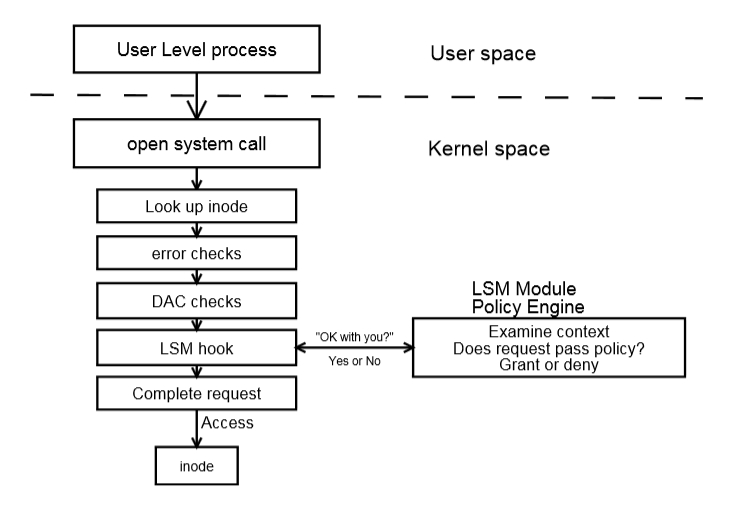
\includegraphics[width=0.9\textwidth]{./images/sec_LSMHook.jpg}
					\caption{Funktionsweise von \emph{\gls{SystemCall}}-Hooks im LSM-Framework \cite[S.3]{LSMFramework}.}
					\label{fig:sec_LSMHook}
			\end{figure}

			Der Ausführungszeitpunkt des Hooks bietet den Vorteil, dass der komplette Kontext der Zugriffsanfrage an dieser Stelle vorliegt und vollständig von einem LSM-Modul ausgewertet werden kann \cite[S.2]{LSMFramework}. Neben der Kompatiblität zum DAC-Mechanismus, wird dadurch zusätzlich die Granularität der Zugriffskontrolle verbessert \cite{LSMDesign}.

			An dieser Stelle ist wichtig zu erwähnen, dass Module des LSM-Frameworks den nativen DAC-Mechanismus nicht überschreiben, sondern ergänzen. Wie in \fig \ref{fig:sec_LSMHook} dargestellt, greift der LSM-Hook erst nachdem ein Nutzer einen sicherheitskritischen \emph{System Call} ausführt hat, das angefragte Objekt aufgelöst, ein Fehler-Check abgeschlossen und der Zugriff über den DAC-Mechanismus genehmigt wurde. Erst wenn der Kernel versucht auf das aufgelöste \glslink{KernelObject}{Kernelobjekt} zuzugreifen, wird der Hook ausgeführt, der den Zugriff in das zugehörige LSM-Modul weiterleitet. Das Modul genehmigt oder verweigert den Zugriff anhand den ihm vorliegenden Attribute im Sicherheitskontext.

			Durch diese Reihenfolge ist sichergestellt, dass die Nutzung einer LSM-Schnittstelle optional ist und unabhängig von der DAC funktioniert \cite{centOsMCS}. Deswegen können auch Anwendungen, die das LSM-Framework nicht unterstützen, weiterhin funktionieren. Außerdem ist durch den rein erweiternden Charakter die Gefahr ausgeschlossen, mit \emph{SELinux} oder \emph{AppArmor} neue Sicherheitslücken in das System einzuführen.
			% logische UND-Verknüpfung von DAC und MAC erwähnen?

			Die Vorgehensweise unterscheidet sich damit grundlegend von der regulären Implementierung einer MAC, da letztere durch ihre obligatorische Natur normalerweise zu Beginn einer Zugriffskontrolle ausgeführt wird \cite[S.3]{LSMFramework}.


			Bei der Verwendung von Sicherheitsmodulen ist auf die Leistungsverluste zu achten, die die einzelnen MACs verursachen. Nach den durchgeführten Benchmarks in \cite[S.51ff.]{SELinuxApparmor} kommt es unter \emph{AppArmor} und \emph{SELinux} bei der Ausführungsgeschwindigkeit der meisten Testoperationen zu Verlusten zwischen 0\% und 11\%. Spezielle Aktionen, wie z.B. das Öffnen und Schließen einer Datei unter \emph{AppArmor}, können die Ausführungszeit verdoppeln.



			Der Sicherheitskontext kann unter Linux für Subjekte mit dem Befehl \texttt{ps} und für Objekte mit dem Befehl \texttt{ls}, jeweils mit dem Parameter \texttt{-Z} ausgegeben werden.

			% lstlisting bringen wo die von Docker-Prozessen und /proc /boot files gekennzeichnet sind

			% TODO: Inhalte aus dem CISSP-Buch (generell MAC im Vgl zu DAC und RBAC). geschlossen, offen. Schwachstellen von DAC (auch schon woanders hier...)

			% Siehe \cite[S.5]{dockerSecIntro} rechts unten

			% Zukuenftiger "security namespace", in dnenen jeder Container seine eigenen LSM/MAC dinger definieren kann, je nach sicherheitsanforderung
			%		^ 	\cite[S.17,18]{dockerSec2}

			% S.7 in



			In den folgenden Unterkapiteln sind die beiden MAC-Implementierungen \emph{AppArmor} und \emph{SELinux} vorgestellt. Exemplarisch wird das Standardprofil von \emph{AppArmor}, das Docker verwendet, im Detail analysiert. Wie sich MACs unter Docker in Zukunft entwickeln, ist im Fazit in Kapitel \ref{result} geschildert.
			% TODO: Checken, ob Referenz wirklich da ist, also Thema in Fazit aufgegriffen ist!

			\subsubsection{\acrshort{AppArmor}}
			\label{apparmor}
      	% Optional, da auf MAC alzu sehr eingehen nicht zu sehr im Scope sein sollte.
				\emph{AppArmor} implementiert eine MAC und wurde als leicht konfigurierbare Alternative zu \emph{SELinux} entwickelt. Es kommt unter den Linux-Distributionen wie \emph{Debian}, \emph{Ubuntu} und \emph{OpenSUSE} standardmäßig zum Einsatz \cite{apparmorUbuntu}.
				% Einfach zu lernen
				% Basiert auf \emph{AppArmor}-Profilen.
				% Es gibt von \emph{Docker} erstelltes Profil, das speziell für den Einsatz von Docker mit \emph{AppArmor} gebaut wurde. \cite{ https://docs.docker.com/engine/articles/security/ }

				Auf Basis von textbasierten Profilen werden anwendungsspezifische Regeln definiert, die den Zugriff auf Objekten über Pfade im Dateisystem und sieben kombinierbare Berechtigungstypen festlegen \cite{linuxSecOverview}\cite{apparmorQuickProfileLanguage}. Durch eine Inkludieranweisung lassen sich mehrere Profile modular kombinieren \cite{apparmorQuickProfileLanguage}.

				Die Sicherheitsziele der Vertrauchlichkeit und Integrität werden über die Berechtigungstypen realisiert: die Datenintegrität kann direkt mit der Verwehrung des Schreibrechts (\texttt{w}) hergestellt werden, während die Vertraulichkeit von Daten auf einem Leseverbot (\texttt{r}) basiert. Dadurch, dass sich z.B. mit einem Schreibvorgang in die Datei \texttt{/proc/sysrq-trigger} das Hostsystem neustarten lässt, haben die zugewiesenen Berechtigungen auch Einfluss auf die Verfügbarkeit.

				% AppArmor profiles can be in one of two modes: enforcement and complain. Profiles loaded in enforcement mode will result in enforcement of the policy defined in the profile as well as reporting policy violation attempts (either via syslog or auditd). Profiles in complain mode will not enforce policy but instead report policy violation attempts.
				% AppArmor differs from some other MAC systems on Linux: it is path-based, it allows mixing of enforcement and complain mode profiles, it uses include files to ease development, and it has a far lower barrier to entry than other popular MAC systems.
				%		^		\cite{ https://wiki.ubuntu.com/AppArmor }

				\emph{AppArmor} unterstützt drei Betriebsmodi, die jeweils folgenden Zweck erfüllen \cite[S.82]{SELinuxApparmor}:
				\begin{itemize}
					\item \emph{Audit}-Modus: Alle erlaubten Zugriffe werden protokolliert.
					\item \emph{Complain}-Modus: Ein Lernmodus, bei dem das Verhalten einer Anwendungen beobachtet wird und aus diesem ein automatisch generiertes Sicherheitsprofil erstellt wird \cite{linuxSecOverview}. In diesem Modus werden Zugriffe, die gegen die Profilregeln verstoßen, nur aufgezeichnet und nicht unterbunden.
					\item \emph{Enforce}-Modus: Die Regeln eines Profils werden erzwungen. Verstöße werden protokolliert.
				\end{itemize}

				% und "sudo aa-status" beweist, dass docker-default im enforce-mode laeuft.
				% TODO: Irgendwo war ein Bild hier von

				Das Docker-Standardprofil \texttt{docker-default} \cite{githubAppArmorProfileContainer}, das im \emph{Enforce}-Modus in nicht-priveligierten Containern zum Einsatz kommt \cite{docker110Security}, wird bei der Installation von Docker in die Datei \texttt{/etc/apparmor.d/docker} geschrieben. Administratoren können sich mit dem Befehl \texttt{sudo aa-status} vergewissern, ob das Standardprofil aktuell aktiv ist. Auch die zurückgegebenen Sicherheitskontexte in der ersten Spalte von \fig \ref{fig:sec_pidNsHost} und \fig \ref{fig:sec_pidNsContainer} belegen die standardmäßige Verwendung von \texttt{docker-default}. Es existiert auch ein Profil für den Docker-Daemon \cite{githubAppArmorProfileDaemon}, allerdings muss dieses manuell aktiviert werden \cite{githubAppArmorDoc}.

				\texttt{docker-default} kann mit dem \texttt{run}-Parameter \texttt{--security-opt="{}apparmor:PROFILE"{}} manuell überschrieben werden, sofern \texttt{PROFILE} zuvor, z.B. mit dem \acrshort{CLI}-Werkzeug \texttt{apparmor\_parser} \cite{apparmorParser}, importiert wurde \cite{dockerRun}.

				%\paragraph{Analyse des Standardprofils}

					Das Standardprofil \texttt{docker-default} wurde während der Erstellung dieser Arbeit aktualisiert. Aus der Commit-Nachricht geht allerdings nicht hervor, ob damit eine Sicherheitslücke geschlossen wurde oder die Änderungen im Zuge einer Funktionsänderung von Containern entstanden sind \cite{githubAppArmorProfileContainerFix}.

					Die aktuelle Implementierung des Profils, die auf einem Docker-Hostsystem lokal mit dem Konsolenbefehl \texttt{cat /etc/apparmor.d/docker} ausgegeben werden kann, wird im Folgenden gruppiert und chronologisch in der Reihenfolge des Vorkommens analysiert.

					\begin{lstlisting}
						#include <tunables/global>
					\end{lstlisting}
					Diese Anweisung inkludiert einige Variablen für die weitere Verwendung. Darunter ist auch die Variable \texttt{@{PROC}} definiert, die in diesem Profil verwendet wird, um das virtuelle Verzeichnis \texttt{/proc/} aufzulösen.

					\begin{lstlisting}
						profile docker-default flags=(attach_disconnected,mediate_deleted) {
							...
						}
					\end{lstlisting}
					Die erste Zeile markiert den Start \texttt{docker-default} mit zwei Flags. Das Flag \texttt{attach\_disconnected} gibt an, dass Verzeichnisse außerhalb eines Namespace direkt in das Rootverzeichnis eingefügt werden \cite{apparmorPolicyReference}. Die Angabe von \texttt{mediate\_deleted} bewirkt eine versuchte Auflösung eines im Speicher gelöschten Objekts anhand dessen Pfad im Dateisystem \cite{apparmorFAQ}. Beide Flags wirken sich nicht direkt auf die Zugriffsverwaltung unter Docker aus und sind nur zur Vollständigkeit erwähnt.

					\begin{lstlisting}
						#include <abstractions/base>
					\end{lstlisting}
					Hiermit werden einige Zugriffsregeln eingebunden, die von fast allen Programm benötigt werden \cite[S.100]{SELinuxApparmor}.

					\begin{lstlisting}
						network,
						capability,
						file,
						umount,
					\end{lstlisting}
					Diese Regeln erlauben die grundsätzliche Verwendung von Netzwerkfunktionen, Capabilities und dem Dateisystem. Außerdem können Mounts mithilfe von \texttt{umount} ausgeworfen werden.

					\begin{lstlisting}
						deny @{PROC}/* w,
					  deny @{PROC}/{[^1-9],[^1-9][^0-9],[^1-9s][^0-9y][^0-9s],[^1-9][^0-9][^0-9][^0-9]*}/** w,
					  deny @{PROC}/sys/[^k]** w,
					  deny @{PROC}/sys/kernel/{?,??,[^s][^h][^m]**} w,
					\end{lstlisting}
					Diese Anweisungen regeln den Schreibzugriff im Verzeichnis \texttt{/proc/}. Effektiv wird das Schreibrecht auf alle Dateien und Verzeichnisse untersagt, die nicht in \texttt{/proc/<number>/} und \texttt{/proc/sys/kernel/shm*} liegen. Erstere, numerischen Verzeichnisse geben Zugriff auf prozessspezifische Daten. Jede Nummer repräsentiert eine Prozess-ID der aktuell laufenden Prozesse. Dateien im Verzeichnis \texttt{/proc/sys/kernel/}, deren Name mit \texttt{shm} beginnt, beziehen sich auf geteilte Speicherbereiche, den \emph{Shared Memory} von Prozessen \cite{apparmorShm}.

					\begin{lstlisting}
						deny @{PROC}/sysrq-trigger rwklx,
					  deny @{PROC}/mem rwklx,
					  deny @{PROC}/kmem rwklx,
					  deny @{PROC}/kcore rwklx,
					\end{lstlisting}
					Mittels dieser Direktiven wird Docker das Lese-, Schreib-, Dateisperrungs-, Linkerzeugungs- und Ausführrecht (in dieser Reihenfolge) für angegebene Dateien verwehrt. Mithilfe von \texttt{sysrq-trigger} können Aktionen programmatisch ausgeführt werden, die auch über die \emph{Magischen S-Abf-Tasten} bewirkt werden können. Darunter fallen u.a. kritische Befehle zur Terminierung von Prozessen oder dem Neustart des Betriebssystems \cite{apparmorMagicSysRQ}\cite{apparmorSysrqTrigger}.

					Die Einträge \texttt{mem}, \texttt{kmem} und \texttt{kcore} beinhalten Speicherbereiche des Kernels.
					% TODO: Quelle dazu... Buch, da online keine richtige quelle ausser stackoverflow existiert

					\begin{lstlisting}
						deny mount,
					\end{lstlisting}
					Diese Zeile verbietet das Einbinden jeglicher Mountpoints.

					\begin{lstlisting}
						deny /sys/[^f]*/** wklx,
						deny /sys/f[^s]*/** wklx,
						deny /sys/fs/[^c]*/** wklx,
						deny /sys/fs/c[^g]*/** wklx,
						deny /sys/fs/cg[^r]*/** wklx,
						deny /sys/firmware/efi/efivars/** rwklx,
						deny /sys/kernel/security/** rwklx,
					\end{lstlisting}
					Diese Liste untersagt, abgesehen von einem Lesezugriff, alle anderen Privilegien aus dem bereits geschilderten Rechteset für das Verzeichnis \texttt{/sys/}. Die Ausnahme bilden effektiv Dateien und Unterverzeichnisse in \texttt{/sys/fs/cgroups/}. Damit ist es Containern möglich Informationen über Control Groups des Hostsystems zu beziehen.

					Zusätzlich darf von Dateien und Unterordnern in \texttt{/sys/firmware/efi/efivars/} und \texttt{/sys/kernel/security} nicht gelesen werden. Das erstgenannte Verzeichnis bietet Informationen über einige Bootvariablen. Zweitgenanntes gewährt Einblick in die aktuelle Konfiguration von Sicherheitsmodulen wie \emph{AppArmor} und \emph{SELinux} \cite{apparmorEFI}\cite{apparmorSecurityFS}\cite{apparmorLWNSecurityFS}.

  		\subsubsection{\acrshort{SELinux}}
			\label{selinux}
      	% Macht Sinn das erst am Ende zu machen, wenn noch Zeit ist. Weil SELinux im Detail mehr Exkurs wird.
				\emph{SELinux} implementiert eine feingranulare MAC, die ursprünglich von der \acrshort{NSA} entwickelt wurde. Es wird verwendet, um mithilfe der Konzepte \emph{Type Enforcement} und \emph{Multi-Level Security} (\acrshort{MLS}) Anforderungen an die Vertraulichkeit und Integrität zu erfüllen \cite{redhatSec}. %\cite[S.201]{learningDocker}.

				Der wesentliche Unterschied zu \emph{AppArmor} ist, dass die Zugriffsverwaltung unter \emph{SELinux} über Label erfolgt, die Subjekten und Objekten in einem Sicherheitskontext angehängt sind.


				Auch unter \emph{SELinux} beruhen die Regeln auf einem Profil, das in diesem Kontext auch Regelwerk genannt wird. Das Regelwerk besteht aus Anweisungen, die konkrete Sicherheitslabel, wie sie im nächsten Abschnitt beschrieben sind, abbilden. Durch die in \fig \ref{fig:sec_SELinux} dargestellte strikte Trennung des Regelwerks und dessen Durchsetzung, lassen sich mit \emph{SELinux} hohe Sicherheitsanforderungen erfüllen. Durch detailreiche Anpassungsmöglichkeiten steht diese MAC unter dem Ruf, schwer konfigurierbar zu sein. \acrshort{GUI}-Werkzeuge, wie \emph{system-config-selinux} und die Bibliothek \emph{libsemanage}, verbessern die Bedienung von \emph{SELinux} und dessen Regelwerken \cite[S.62,67]{linuxMagazineSec}.
				% cite { https://www.linux.com/learn/docs/727873-overview-of-linux-kernel-security-features/ }
				% cite { https://www.nsa.gov/research/_files/selinux/papers/selsymp2006.pdf }

				\emph{SELinux} kennt das Konzept der DAC von Besitzern und Gruppen nicht. Der komplette Funktionsumfang von \emph{SELinux} beruht auf einem Labelingsystem, das Zugriffe individuell für Subjekte verwaltet \cite{SELinuxComic}. In Zuge dessen wird jedem Subjekt zur Laufzeit und jedem Objekt im System ein Label nach dem Schema \texttt{User:Role:Type:Level} zugewiesen \cite{atomicDockerSELinux}. Die erste Komponente \texttt{User} eines Labels ist von einem Nutzer unter Linux unabhängig.

				\begin{figure}[h]
						\centering
						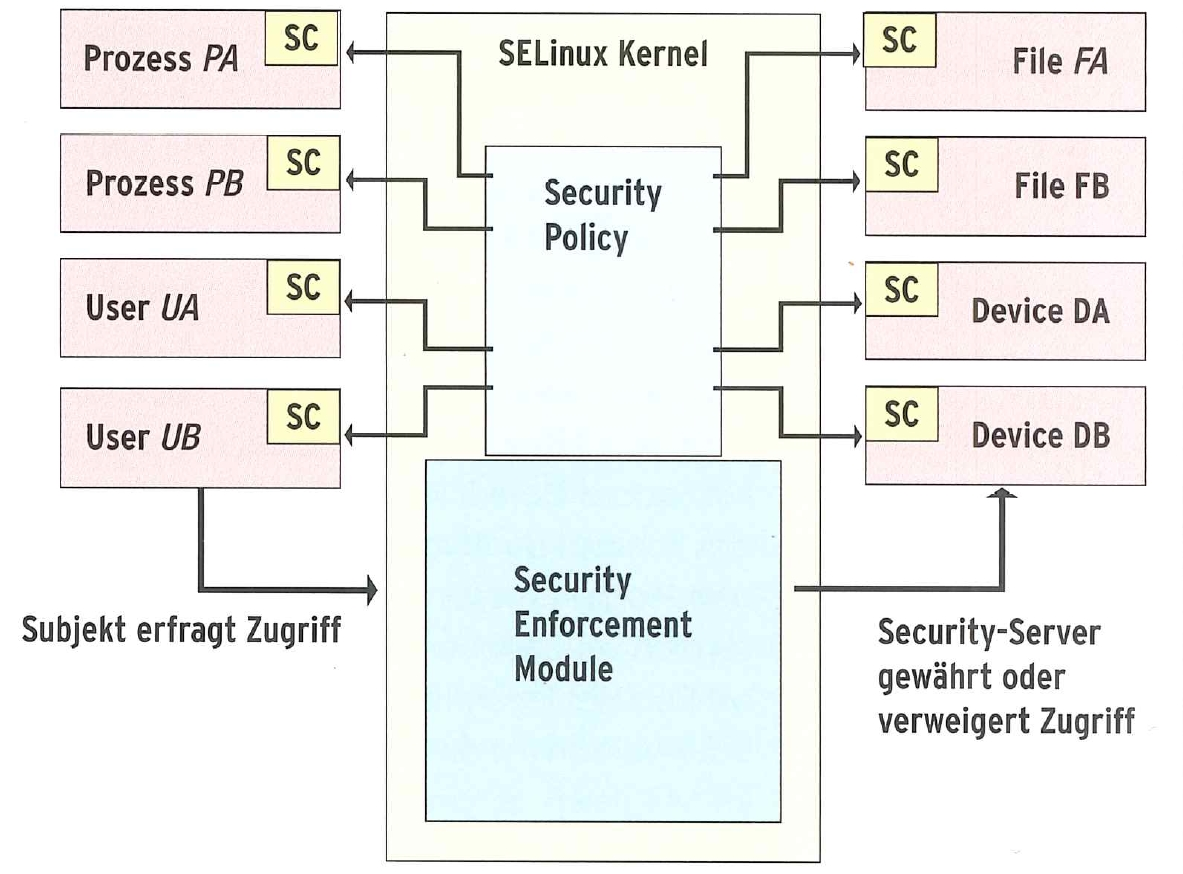
\includegraphics[width=0.9\textwidth]{./images/sec_SELinux.jpg}
						\caption{Trennung von Regelwerk und Enforcement-Modul. Zuweisung von Security-Contexts (SC) an Objekte und Subjekte \cite[S.63]{linuxMagazineSec}.}
						\label{fig:sec_SELinux}
				\end{figure}

				Das Label ist in die erweiternden Attribute (\texttt{xattr}) von Subjekten und Objekten geschrieben \cite[S.65]{linuxMagazineSec}. In \fig \ref{fig:sec_SELinux} ist das Label als \emph{SC} (Security-Context) illustriert.

				% TODO: SELinux profile unter https://github.com/docker/docker/tree/master/contrib/docker-engine-selinux
				% (ist es wirklich das richtige? das ist in /contrib?) aber evtl auch kompiliert iwo im deb/rpm package mit drin..)
				% |
				% Such a policy is written using a .te file (type enforcement) and an optional .fc file (file contexts) and .if file (interfaces).
				%		^		\cite{https://wiki.gentoo.org/wiki/SELinux/Tutorials/Creating_your_own_policy_module_file}

				\emph{SELinux} wertet bei einem Zugriff das Label des zugreifenden Prozesses und das Label der betroffenen Ressource anhand einem definierten Regelwerk aus und entscheidet, ob die Operation fortgesetzt werden darf \cite{linuxSecOverview}.

				Wie unter \emph{AppArmor}, bietet auch \emph{SELinux} Möglichkeiten zum Logging von Zugriffen an.
				% TODO: QUelle

				Die Linux-Distributionen \emph{Red Hat Enterprise Linux}, \emph{Fedora} und \emph{CentOS} verwenden \emph{SELinux} standardmäßig \cite{dockerSecurity}. Unter anderen Distributionen wie \emph{Debian} und \emph{Ubuntu} kann \emph{SELinux} manuell installiert werden \cite{selinuxDebian}\cite{selinuxUbuntu}.

				Seit November 2015 Docker unter dem Release 1.9 mit einer standardmäßigen \emph{SELinux}-Policy ausgestattet \cite{githubDockerChangelog}\cite{githubSELinuxPolicyIssue}.
				%, die in dem \emph{rpm}-basierten Distributionen wie \emph{CentOS} und \emph{Fedora} verwendet wird.
				 Dieses standardmäßige Regelwerk kann über \cite{githubSELinuxProfile} aufgerufen werden.

				Unter Docker können die vier Labelattribute mit dem Parameter \texttt{--security-opt="{}label:LABEL:VALUE"{}} für den \texttt{run}-Befehl pro Container manuell spezifiziert werden \cite{dockerRun}.



				Auf eine Anwendung abgestimmtes \emph{SELinux}-Regelwerk wird mit der sicherheitskritischen Anwendung zusammen verteilt. Bei der Installation wird dann auch die anwendungsspezifische Regelwerk in das LSM geladen, sodass der Sicherheitsmechanismus nicht manuell administriert werden muss. Das Regelwerk bei der ersten Verwendung der Anwendung sofort aktiv.

				Die Funktionsweise zweier \emph{SELinux}-Bausteine, \emph{Type Enforcement} und \emph{Multi-Category Security}, werden im Folgenden erklärt. Ein dritter Baustein, \emph{Multi-Level Security}, wird in dieser Arbeit nicht behandelt, da dieser unter Docker keine Verwendung findet.
				% Multi-Level Security (MLS) ist verwandt mit MCS. Aber kein Einsatz unter Docker. MLS beruht auf Konzept von "Domination".

				% SELinux funktionert angeblich nicht mit storage driver BRTFS		--> s. auch docker version 1.10 release notes unter security headline
				%		^		\cite{ https://coreos.com/blog/container-security-selinux-coreos.html } --> "notes for deploying"

				% Trennung von Zugriffsdomänen auf zwei Ebenen (TE und MCS)
				%(		^		\cite{learning docker book, see https://books.google.de/books?id=jkkOCgAAQBAJ&pg=PA200&lpg=PA200&dq=mcs+docker&source=bl&ots=0mWUrsFsfO&sig=UXFaVbKKMMXcb_nFW-abQeR0bB0&hl=de&sa=X&ved=0ahUKEwiq5pnLltnKAhUGqA4KHY13AqsQ6AEIXjAI#v=onepage&q=mcs%20docker&f=false .... seite 201}

				% TODO: https://coreos.com/blog/container-security-selinux-coreos.html

				\paragraph{Type Enforcement (TE)}
					Die wichtigste Komponente von \emph{SELinux} ist das \emph{Type Enforcement}. Im Rahmen dieses Konzepts werden jedem Subjekt und jedem Objekt ein Typ zugeweisen, deren Auswertung bei jeder Zugriffsoperation zwischen Subjekt und Objekt stattfindet. Der Typ ist im Label an dritter Stelle definiert.

					In der Praxis existieren für jede Anwendung eigene Typen, da jede Anwendung spezielle Rechte benötigt, um ihre Funktion zu erfüllen. Jedem Docker-Prozess ist z.B. der Typ \texttt{docker\_t} zugewiesen, der gleichzeitig eine gemeinsame Domäne für besagte Prozesse definiert. Im \emph{SELinux}-Regelwerk ist festgelegt, dass Prozesse eines Typs nur auf Objekte vollen Zugriff hat, die mit bestimmten Labeltypen versehen sind. Im konkreten Fall von \texttt{docker\_t} umfasst diese Konfiguration ein Objektset, das u.a. aus den Typen \texttt{docker\_config\_t}, \texttt{docker\_log\_t} und \texttt{svirt\_sandbox\_file\_t} besteht \cite{githubSELinuxProfileTE}. Versucht ein Docker-Prozess auf Objekte zuzugreifen, deren Typ nicht in \cite{githubSELinuxProfileTE} gelistet ist, wird die Operation unterbunden.

					Da in \emph{SELinux}-Umgebungen jedem Objekt im Hostsystem ein Label zugewiesen ist, wird eine zuverlässige Kontrolle von Objektzugriffen über die Auswertung von Typen ermöglicht. Subjekte, die mit dem Typ \texttt{docker\_t} aus der Docker-Domäne stammen, sind streng von Objekten anderer Domänen abgegrenzt und können nicht mit diesen interagieren.

				\paragraph{Multi-Category Security (MCS)}
					% TODO: Einarbeiten, dass mit Kateogiren die Vertraulichkeit erfüllt wird: Kategorisierung führt dazu, dass nur solche Prozesse auf Objekte haben, die derselben Kategorie angehören.
					% TODO: Systemintegrität und Domänen mit Type Enforcement realisiert! Prozesse laufen innerhalb einer Domäne und Objekte haben einen Typ. Durch Regeln wird bestimmt, welche Domänen auf welche Typen zugreifen dürfen.
					Durch das einheitliche Regelwerk für alle Docker-Prozesse, ist mit einem \emph{Type Enforcement} gewährleistet, dass ein kompromittierter Container \cbroken{} nicht unbefugt auf geschützte oder unrelevante Daten außerhalb der Docker-Domäne  zugreifen darf. Docker-unspezifische Subjekte und Objekte werden dadruch im Hostsystem geschützt.

					MCS implementiert eine Möglichkeit, \cbroken{} den Zugriff auf \cvalid zu verweigern. Mit \emph{Type Enforcement} ist das nicht realisierbar, da \cbroken{} und \cvalid{} beide durch den identischen Typ \texttt{docker\_t} der Docker-Domäne zugehörig sind.

					Theoretisch wäre die Funktion der MCS auch mit dem\emph{Type Enforcement} realisierbar, wenn jeder Container mit einem eigenen Typ operiert. Die Domäne würde dabei nicht für alle Docker-Subjekte gelten, sondern nur für solche eines Containers. Diese feinere Typenunterteilung wirkt sich aber auf die Komplexität des Regelwerks negativ aus. In der Praxis wird deswegen der MCS-Mechanismus für dieses Sicherheitsfeature eingesetzt.
					% TODO: Quelle!
					% ist aber sehr aufwendig...


					Der MCS-Mechanismus arbeitet mit dem letzten Teil des Labels: dem Level. Das Level unterteilt sich durch den Aufbau der Schreibweise \texttt{sensitivity[:category-set]} in eine Sensitivität, oder auch Schutzstufe genannt, und optionalen Kategorien. Für die MCS sind die Kategorien von Bedeutung. Die Schutzstufe wird ignoriert, weil sie nur unter der von Docker nicht verwendeten \acrshort{MLS} Anwendung findet. Im Fall von Docker hat die Schutzstufe deswegen einen konstanten Wert von \texttt{s0} \cite{selinuxRedhatMCS}\cite{selinuxRedhatMCS}.
					% Quellen!
					%\cite{ https://access.redhat.com/documentation/en-US/Red_Hat_Enterprise_Linux/6/html/Security-Enhanced_Linux/chap-Security-Enhanced_Linux-SELinux_Contexts.html } \cite{ http://james-morris.livejournal.com/5583.html }

					Beim Startvorgang eines Containers wird diesem eine zufällige Kategorie anhand einer Nummer zwischen 0 und 1023 zugeweisen. Diese Kategorie, z.B. nach obiger Syntax \texttt{c623}, wird daraufhin auch vom Docker-Daemon auf den Inhalt containerspezifischer Verzeichnisse angewandt. Sobald während des Betriebs ein Container den Zugriff auf ein Objekt fordert, wird seine Kategorie mit dem des angefragten Objekts verglichen. Stimmen diese überein, ist die MCS-Kontrolle erfolgreich und der Zugriff wird freigegeben. Die Sicherheit von MCS unter Docker beruht auf der Annahme, dass der Docker-Daemon zuverlässig eindeutige Kategorien an die Container vergibt \cite[S.200f.]{learningDocker}.
					% Quelle!
					% \cite{learningDocker}.


					% Quelle!
					% war glaub ich auch aus learningDocker....s201

					Damit erfüllt MCS die zuvor beschriebene Anforderung. Einem \cbroken{} ist es ihm Rahmen einer korrekt implementierten MCS unter \emph{SELinux} nicht mehr möglich, Schaden an zu schützenden Containern aus \(C\) auszuüben.
					% Verständnisproblem: Auch wenn Angreifer Root-Rechte erwirkt? Ist er dann noch "im Container"?


					% n computer systems we often have lots of processes all with the same access, but we want them separated from each other. We sometimes call this a multi-tenant environment. The best example of this is virtual machines. If I have a server running lots of virtual machines, and one of them gets hacked, I want to prevent it from attacking the other virtual machines and virtual machine images. But in a type enforcement system the KVM virtual machine is labeled svirt_t and the image is labeled svirt_image_t. We have rules that say svirt_t can read/write/delete content labeled svirt_image_t. With libvirt we implemented not only type enforcement separation, but also MCS separation. When libvirt is about to launch a virtual machine it picks out a random MCS label like s0:c1,c2, it then assigns the svirt_image_t:s0:c1,c2 label to all of the content that the virtual machine is going to need to manage. Finally, it launches the virtual machine as svirt_t:s0:c1,c2. Then, the SELinux kernel controls that svirt_t:s0:c1,c2 can not write to svirt_image_t:s0:c3,c4, even if the virtual machine is controled by a hacker and takes it over. Even if it is running as root.

					% We use similar separation in OpenShift. Each gear (user/app process)runs with the same SELinux type (openshift_t). Policy defines the rules controlling the access of the gear type and a unique MCS label to make sure one gear can not interact with other gears.

				%\paragraph{Multi-Level Security (MLS)}
					%\emph{DELETE -- MLS nicht unter Docker genutzt...}
					% Arbeitet MLS nur auf s0...sX ebene und ignoriert c0..cX?

					% MLS enforces the Bell-La Padula Mandatory Access Model
					%		^		\cite{ https://access.redhat.com/documentation/en-US/Red_Hat_Enterprise_Linux/6/html/Security-Enhanced_Linux/chap-Security-Enhanced_Linux-SELinux_Contexts.html }

					% I could have two Apache servers: one running as httpd_t:TopSecret and another running as httpd_t:Secret. If the Apache process httpd_t:Secret were hacked, the hacker could read httpd_sys_content_t:Secret but would be prevented from reading httpd_sys_content_t:TopSecret.

					% However, if the Apache server running httpd_t:TopSecret was hacked, it could read httpd_sys_content_t:Secret data as well as httpd_sys_content_t:TopSecret.

					% We use the MLS in military environments where a user might only be allowed to see secret data, but another user on the same system could read top secret data.

					%------

					% The Multi-Level Security technology refers to a security scheme that enforces the Bell-La Padula Mandatory Access Model. Under MLS, users and processes are called subjects, and files, devices, and other passive components of the system are called objects. Both subjects and objects are labeled with a security level, which entails a subject's clearance or an object's classification. Each security level is composed of a sensitivity and a category, for example, an internal release schedule is filed under the internal documents category with a confidential sensitivity.


    \subsection{Seccomp}
		\label{seccomp}
			% TODO: https://lwn.net/Articles/443099/ und https://lwn.net/Articles/441232/
			% TODO: und vllt https://lwn.net/Articles/443110/

			% TODO: https://blog.docker.com/2016/02/docker-online-meetup-33-security/ ... slide 12+13 (s.13 mit links) ... die acions aufzaehlen und welche von doker im standardprofil verwendet werden.
			% da auch drin: CVE prevented

			\emph{Seccomp} steht für \emph{Secure Computing Mode} und setzt einen von \emph{Google} implementierten Mechanismus um, der den Zugriff von Prozessen auf \emph{System Calls} einschränkt. Die Idee von \emph{Seccomp} ist es, die Angriffsfläche des Kernels zu minimieren, indem für Anwendungen bestimmte \emph{System Calls}  blockiert werden. Die Gefahr, dass fehlerbehaftete oder unsichere \emph{System Calls} genutzt werden, die die Anwendung zum fehlerfreien Betrieb nicht benötigt, wird dadurch reduziert \cite{linuxSecOverview}\cite{seccompGitDesc}\cite{secInFuture}.

			\emph{Seccomp} ist nicht wie \emph{SELinux} und \emph{AppArmor} als LSM implementiert \cite{seccompLWN}.
			% \emph{SO NICHT RICHTIG, siehe https://github.com/docker/docker/blob/master/docs/security/seccomp.md}.
			%	Secure computing mode (Seccomp) is a Linux kernel feature. You can use it to restrict the actions available within the container. The seccomp() system call operates on the seccomp state of the calling process. You can use this feature to restrict your application's access.
			% This feature is available only if the kernel is configured with CONFIG_SECCOMP enabled.

			%Das hat die positive Auswirkung, dass \emph{Seccomp}-Profile auch von nicht-priveligierten Nutzern geladen werden können. Mit LSMs ist dies nicht möglich.
			% 	^		\cite{ https://lwn.net/Articles/443099/ }
			Die Verwendung von \emph{Seccomp} für einen Prozess bewirkt, dass dieser in einen \glqq{}sicheren\grqq{} Zustand übergeht, sodass er nur noch zuvor definierte \emph{System Calls} ausführen kann.
			%		^		\cite{ wikipedia :( }

			% x86_x64 hat mehr als 600 System Calls. bzw. mehrere hundert
			%		^		\cite{ https://opensource.com/business/15/3/docker-security-future }

			% This feature is available only if the kernel is configured with CONFIG_SECCOMP enabled.
			%		^		\cite{ https://github.com/docker/docker/blob/master/docs/security/seccomp.md }

			Das originale Seccomp, auch als \emph{Mode 1} bekannt, stellt nur den Zugriff auf vier \emph{System Calls} zur Verfügung: \texttt{read}, \texttt{write}, \texttt{exit} und \texttt{sigreturn}. Diese vier Aufrufe repräsentieren ein minimales Set an Operationen, die eine nicht vertrauenswürdige Anwendung ausführen darf \cite{linuxSecOverview}.

			Ein Update \emph{Mode 2} macht das Set an erlaubten \emph{System Calls} mithilfe von Filtern frei konfigurierbar und führt ein \emph{Audit Logging} ein	\cite{linuxSecOverview}\cite{seccompGitDesc}.

			Mithilfe der \emph{Seccomp}-Anweisungen \texttt{allow}, \texttt{deny}, \texttt{trap}, \texttt{kill} und \texttt{trace} sind neben der Sperrung noch weitere Aktionen möglich, die zur Kontrolle von \emph{System Calls} dienen \cite{docker110Security}.

			Seit Oktober 2015 ist eine \emph{Seccomp}-Unterstützung für Docker in Planung und Entwicklung \cite{githubGeneralSecProfiles}\cite{githubSeccompIntegration}. Diese wurde in Form eines \emph{Seccomp}-Standardprofils und der Option eigene Profile einzubinden, in aktuell neusten Docker-Version 1.10 im Februar 2016, hinzugefügt \cite{githubDockerChangelog}\cite{githubSeccompDoc}\cite{githubSeccompProfile}\cite{docker110Security}. Das Standardprofil basiert seit Ende 2015 auf einer Whitelist (davor einer Blacklist). Dadurch blockiert es alle \emph{System Calls}, die nicht in der Whitelist als erlaubte Operationen aufgeführt sind \cite{githubSeccompDoc}.

			Eine aktuelle Liste der explizit erlaubten \emph{System Calls} ist in \cite{githubSeccompProfile} und \cite{githubSeccompDoc} zu finden.

			Seit der Umstellung von Blacklisting auf Whitelisting wurde die \emph{System Call}-Auflistung in einem Zeitraum von ca. fünf Wochen 47 Änderungen unterzogen. Davon sind 40 Neueinträge und sieben Löschungen zu registrieren \cite{githubSeccompProfileHistory}. Während es sich bei den Neueinträgen um bewusste Funktionserweiterungen handeln kann, werfen sieben Löschungen den Verdacht auf, dass das \emph{Seccomp}-Standardprofil weder als vollständig noch ausreichend getestet, betrachtet werden kann.
			% (TODO): CHECK AGAIN nach commit history aenderungen!

			Die offizielle Dokumentation des \texttt{run}-Befehls sieht noch keine Anpassungsmöglichkeit von \emph{Seccomp} vor \cite{dockerRun}. Jedoch ist an anderer Stelle im \emph{GitHub}-Repository vermerkt, dass sich das Standardprofil mit dem Parameter \texttt{--security-opt seccomp:PROFILEPATH} überschreiben lässt \cite{githubSeccompDoc}. Ist es nötig, Container ohne \emph{Seccomp} zu starten, kann das mit der Option \texttt{--security-opt seccomp:unconfined} realisiert werden \cite{dockerRun}\cite{docker110Security}.

	%\section{Docker im Vergleich zu anderen Containerlösungen}
  	% Optional?

		% Vergleich von CoreOs 1.0 und Docker 1.10?

		% Selbst steinaltes OpenBSD baut noch an tame() / neu:pledge() -Funktion rum, um soetwas wie Seccomp zu ermoeglichen
		%	Tame() als Vorbild fuer general framework von docker (siehe RFC github post von frazelli) --> Mehr in Fazit-Kapitel rein.
		%		^		\cite{https://news.ycombinator.com/item?id=10537268}

		% Von CoreOS-Website: Security-minded capabilities
		% rkt is built from the ground up to be ready for security-focused environments. Many of these principles weren’t invented at CoreOS — instead, we applied common, everyday best practices that have been largely overlooked in the container industry so far.

\end{document}
